\documentclass[pdflatex,11pt]{dokumentacja}
\usepackage[polish]{babel}
\usepackage[utf8]{inputenc}

% dodatkowe pakiety
\usepackage{enumerate}
\usepackage{listings}
\usepackage{hyperref}
\usepackage{fancyvrb}
\usepackage{color}
\usepackage{float}

\floatstyle{ruled}
\newfloat{program}{thp}{lop}
\floatname{program}{Kod źródłowy}
\newenvironment{code}{\selectfont\small}{\par}

\lstloadlanguages{TeX}
\hypersetup{%
    pdfborder = {0 0 0}
}
%---------------------------------------------------------------------------

\author{Paweł Kaczmarczyk, Stanisław Podgórski}
\shortauthor{P. Kaczmarczyk, S. Podgórski}

\titlePL{Rozproszony system do testowania algorytmów planowania: Serwisy wykonujące planowanie przy pomocy różnych algorytmów}

\shorttitlePL{Serwisy wykonywujące planowanie przy pomocy różnych algorytmów}

\thesistypePL{Zaawansowane techniki integracji systemów}

\date{2013}

\departmentPL{Katedra Informatyki}

\facultyPL{Wydział Informatyki, Elektroniki i Telekomunikacji}

\setlength{\cftsecnumwidth}{10mm}

%---------------------------------------------------------------------------

\begin{document}

\titlepages

\include{abstract}

\tableofcontents

\listoffigures 

\clearpage

\chapter{Cel projektu}

Celem realizowanego projektu było:

\begin{itemize}
	\item Udostepnienie serwisu odszukiwania scieżek w grafach.
	\item Umożliwienie wyboru różnych algorytmów planowania.
	\item Udostępnienie statystyk do ewaluacji dostarczanych algorytmów.
\end{itemize}

Serwis miał otrzymywać zlecenia w postaci grafu oraz węzła początkowego i końcowego, a następnie zwracać ścieżkę pomiędzy tymi punktami oraz meta-informacje związane z procesem obliczania ścieżki.

\section{Poszukiwanie ścieżek}

Problem poszukiwania możliwie optymalnej ścieżki w grafie sprowadza się do wyznaczenia zbioru węzłów lub zbioru krawędzi (istotne dla multigrafów) poprzez które można dostać się z węzła początkowego do węzła końcowego.
Interesują nas zwykle ścieżki, dla których sumaryczna wartość wag mijanych krawędzi będzie najmniejsza.
Rysunek \ref{fig:planowanie} przedstawia działanie algorytmu planowania dla przykładowego garfu.

\begin{figure}[!h]
	\centering
	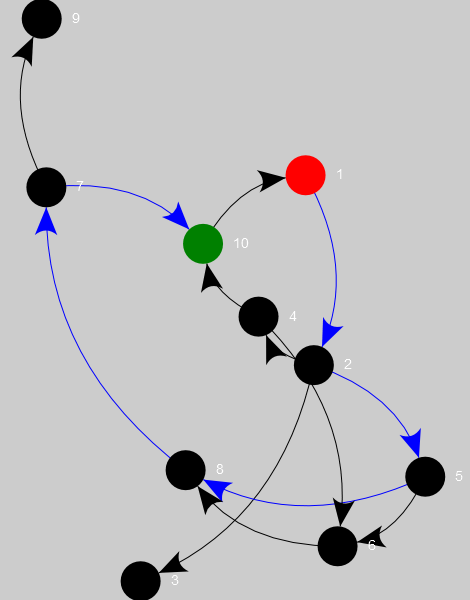
\includegraphics{img/planowanie.png}
	\caption{Przykład wyszukiwania ścieżki w grafie.}
	\label{fig:planowanie}
\end{figure}

\section{Motywacja projektu}

Stworzony system może zostać wykorzystany w kilku różnych scenariuszach użycia:
\begin{itemize}
	\item Ewaluacja działania różnych algorytmów dla wybranego typu grafów.
	\item Ewaluacja wybranego algorytmu planowania dla różnych rodzajów grafów.
	\item Określenie wymagań czasowych i pamięciowych dla konkretnych problemów planowania
\end{itemize}
\chapter{Wymagania}

\section{Wymagania funkcjonalne}

\section{Wymagania niefunkcjonalne}
\chapter{Wizja}

\section{Wstępna}

\section{Końcowa}
\makeatletter
\def\PY@reset{\let\PY@it=\relax \let\PY@bf=\relax%
    \let\PY@ul=\relax \let\PY@tc=\relax%
    \let\PY@bc=\relax \let\PY@ff=\relax}
\def\PY@tok#1{\csname PY@tok@#1\endcsname}
\def\PY@toks#1+{\ifx\relax#1\empty\else%
    \PY@tok{#1}\expandafter\PY@toks\fi}
\def\PY@do#1{\PY@bc{\PY@tc{\PY@ul{%
    \PY@it{\PY@bf{\PY@ff{#1}}}}}}}
\def\PY#1#2{\PY@reset\PY@toks#1+\relax+\PY@do{#2}}

\expandafter\def\csname PY@tok@gd\endcsname{\def\PY@tc##1{\textcolor[rgb]{0.63,0.00,0.00}{##1}}}
\expandafter\def\csname PY@tok@gu\endcsname{\let\PY@bf=\textbf\def\PY@tc##1{\textcolor[rgb]{0.50,0.00,0.50}{##1}}}
\expandafter\def\csname PY@tok@gt\endcsname{\def\PY@tc##1{\textcolor[rgb]{0.00,0.27,0.87}{##1}}}
\expandafter\def\csname PY@tok@gs\endcsname{\let\PY@bf=\textbf}
\expandafter\def\csname PY@tok@gr\endcsname{\def\PY@tc##1{\textcolor[rgb]{1.00,0.00,0.00}{##1}}}
\expandafter\def\csname PY@tok@cm\endcsname{\let\PY@it=\textit\def\PY@tc##1{\textcolor[rgb]{0.25,0.50,0.50}{##1}}}
\expandafter\def\csname PY@tok@vg\endcsname{\def\PY@tc##1{\textcolor[rgb]{0.10,0.09,0.49}{##1}}}
\expandafter\def\csname PY@tok@m\endcsname{\def\PY@tc##1{\textcolor[rgb]{0.40,0.40,0.40}{##1}}}
\expandafter\def\csname PY@tok@mh\endcsname{\def\PY@tc##1{\textcolor[rgb]{0.40,0.40,0.40}{##1}}}
\expandafter\def\csname PY@tok@go\endcsname{\def\PY@tc##1{\textcolor[rgb]{0.53,0.53,0.53}{##1}}}
\expandafter\def\csname PY@tok@ge\endcsname{\let\PY@it=\textit}
\expandafter\def\csname PY@tok@vc\endcsname{\def\PY@tc##1{\textcolor[rgb]{0.10,0.09,0.49}{##1}}}
\expandafter\def\csname PY@tok@il\endcsname{\def\PY@tc##1{\textcolor[rgb]{0.40,0.40,0.40}{##1}}}
\expandafter\def\csname PY@tok@cs\endcsname{\let\PY@it=\textit\def\PY@tc##1{\textcolor[rgb]{0.25,0.50,0.50}{##1}}}
\expandafter\def\csname PY@tok@cp\endcsname{\def\PY@tc##1{\textcolor[rgb]{0.74,0.48,0.00}{##1}}}
\expandafter\def\csname PY@tok@gi\endcsname{\def\PY@tc##1{\textcolor[rgb]{0.00,0.63,0.00}{##1}}}
\expandafter\def\csname PY@tok@gh\endcsname{\let\PY@bf=\textbf\def\PY@tc##1{\textcolor[rgb]{0.00,0.00,0.50}{##1}}}
\expandafter\def\csname PY@tok@ni\endcsname{\let\PY@bf=\textbf\def\PY@tc##1{\textcolor[rgb]{0.60,0.60,0.60}{##1}}}
\expandafter\def\csname PY@tok@nl\endcsname{\def\PY@tc##1{\textcolor[rgb]{0.63,0.63,0.00}{##1}}}
\expandafter\def\csname PY@tok@nn\endcsname{\let\PY@bf=\textbf\def\PY@tc##1{\textcolor[rgb]{0.00,0.00,1.00}{##1}}}
\expandafter\def\csname PY@tok@no\endcsname{\def\PY@tc##1{\textcolor[rgb]{0.53,0.00,0.00}{##1}}}
\expandafter\def\csname PY@tok@na\endcsname{\def\PY@tc##1{\textcolor[rgb]{0.49,0.56,0.16}{##1}}}
\expandafter\def\csname PY@tok@nb\endcsname{\def\PY@tc##1{\textcolor[rgb]{0.00,0.50,0.00}{##1}}}
\expandafter\def\csname PY@tok@nc\endcsname{\let\PY@bf=\textbf\def\PY@tc##1{\textcolor[rgb]{0.00,0.00,1.00}{##1}}}
\expandafter\def\csname PY@tok@nd\endcsname{\def\PY@tc##1{\textcolor[rgb]{0.67,0.13,1.00}{##1}}}
\expandafter\def\csname PY@tok@ne\endcsname{\let\PY@bf=\textbf\def\PY@tc##1{\textcolor[rgb]{0.82,0.25,0.23}{##1}}}
\expandafter\def\csname PY@tok@nf\endcsname{\def\PY@tc##1{\textcolor[rgb]{0.00,0.00,1.00}{##1}}}
\expandafter\def\csname PY@tok@si\endcsname{\let\PY@bf=\textbf\def\PY@tc##1{\textcolor[rgb]{0.73,0.40,0.53}{##1}}}
\expandafter\def\csname PY@tok@s2\endcsname{\def\PY@tc##1{\textcolor[rgb]{0.73,0.13,0.13}{##1}}}
\expandafter\def\csname PY@tok@vi\endcsname{\def\PY@tc##1{\textcolor[rgb]{0.10,0.09,0.49}{##1}}}
\expandafter\def\csname PY@tok@nt\endcsname{\let\PY@bf=\textbf\def\PY@tc##1{\textcolor[rgb]{0.00,0.50,0.00}{##1}}}
\expandafter\def\csname PY@tok@nv\endcsname{\def\PY@tc##1{\textcolor[rgb]{0.10,0.09,0.49}{##1}}}
\expandafter\def\csname PY@tok@s1\endcsname{\def\PY@tc##1{\textcolor[rgb]{0.73,0.13,0.13}{##1}}}
\expandafter\def\csname PY@tok@sh\endcsname{\def\PY@tc##1{\textcolor[rgb]{0.73,0.13,0.13}{##1}}}
\expandafter\def\csname PY@tok@sc\endcsname{\def\PY@tc##1{\textcolor[rgb]{0.73,0.13,0.13}{##1}}}
\expandafter\def\csname PY@tok@sx\endcsname{\def\PY@tc##1{\textcolor[rgb]{0.00,0.50,0.00}{##1}}}
\expandafter\def\csname PY@tok@bp\endcsname{\def\PY@tc##1{\textcolor[rgb]{0.00,0.50,0.00}{##1}}}
\expandafter\def\csname PY@tok@c1\endcsname{\let\PY@it=\textit\def\PY@tc##1{\textcolor[rgb]{0.25,0.50,0.50}{##1}}}
\expandafter\def\csname PY@tok@kc\endcsname{\let\PY@bf=\textbf\def\PY@tc##1{\textcolor[rgb]{0.00,0.50,0.00}{##1}}}
\expandafter\def\csname PY@tok@c\endcsname{\let\PY@it=\textit\def\PY@tc##1{\textcolor[rgb]{0.25,0.50,0.50}{##1}}}
\expandafter\def\csname PY@tok@mf\endcsname{\def\PY@tc##1{\textcolor[rgb]{0.40,0.40,0.40}{##1}}}
\expandafter\def\csname PY@tok@err\endcsname{\def\PY@bc##1{\setlength{\fboxsep}{0pt}\fcolorbox[rgb]{1.00,0.00,0.00}{1,1,1}{\strut ##1}}}
\expandafter\def\csname PY@tok@kd\endcsname{\let\PY@bf=\textbf\def\PY@tc##1{\textcolor[rgb]{0.00,0.50,0.00}{##1}}}
\expandafter\def\csname PY@tok@ss\endcsname{\def\PY@tc##1{\textcolor[rgb]{0.10,0.09,0.49}{##1}}}
\expandafter\def\csname PY@tok@sr\endcsname{\def\PY@tc##1{\textcolor[rgb]{0.73,0.40,0.53}{##1}}}
\expandafter\def\csname PY@tok@mo\endcsname{\def\PY@tc##1{\textcolor[rgb]{0.40,0.40,0.40}{##1}}}
\expandafter\def\csname PY@tok@kn\endcsname{\let\PY@bf=\textbf\def\PY@tc##1{\textcolor[rgb]{0.00,0.50,0.00}{##1}}}
\expandafter\def\csname PY@tok@mi\endcsname{\def\PY@tc##1{\textcolor[rgb]{0.40,0.40,0.40}{##1}}}
\expandafter\def\csname PY@tok@gp\endcsname{\let\PY@bf=\textbf\def\PY@tc##1{\textcolor[rgb]{0.00,0.00,0.50}{##1}}}
\expandafter\def\csname PY@tok@o\endcsname{\def\PY@tc##1{\textcolor[rgb]{0.40,0.40,0.40}{##1}}}
\expandafter\def\csname PY@tok@kr\endcsname{\let\PY@bf=\textbf\def\PY@tc##1{\textcolor[rgb]{0.00,0.50,0.00}{##1}}}
\expandafter\def\csname PY@tok@s\endcsname{\def\PY@tc##1{\textcolor[rgb]{0.73,0.13,0.13}{##1}}}
\expandafter\def\csname PY@tok@kp\endcsname{\def\PY@tc##1{\textcolor[rgb]{0.00,0.50,0.00}{##1}}}
\expandafter\def\csname PY@tok@w\endcsname{\def\PY@tc##1{\textcolor[rgb]{0.73,0.73,0.73}{##1}}}
\expandafter\def\csname PY@tok@kt\endcsname{\def\PY@tc##1{\textcolor[rgb]{0.69,0.00,0.25}{##1}}}
\expandafter\def\csname PY@tok@ow\endcsname{\let\PY@bf=\textbf\def\PY@tc##1{\textcolor[rgb]{0.67,0.13,1.00}{##1}}}
\expandafter\def\csname PY@tok@sb\endcsname{\def\PY@tc##1{\textcolor[rgb]{0.73,0.13,0.13}{##1}}}
\expandafter\def\csname PY@tok@k\endcsname{\let\PY@bf=\textbf\def\PY@tc##1{\textcolor[rgb]{0.00,0.50,0.00}{##1}}}
\expandafter\def\csname PY@tok@se\endcsname{\let\PY@bf=\textbf\def\PY@tc##1{\textcolor[rgb]{0.73,0.40,0.13}{##1}}}
\expandafter\def\csname PY@tok@sd\endcsname{\let\PY@it=\textit\def\PY@tc##1{\textcolor[rgb]{0.73,0.13,0.13}{##1}}}

\def\PYZbs{\char`\\}
\def\PYZus{\char`\_}
\def\PYZob{\char`\{}
\def\PYZcb{\char`\}}
\def\PYZca{\char`\^}
\def\PYZam{\char`\&}
\def\PYZlt{\char`\<}
\def\PYZgt{\char`\>}
\def\PYZsh{\char`\#}
\def\PYZpc{\char`\%}
\def\PYZdl{\char`\$}
\def\PYZhy{\char`\-}
\def\PYZsq{\char`\'}
\def\PYZdq{\char`\"}
\def\PYZti{\char`\~}
% for compatibility with earlier versions
\def\PYZat{@}
\def\PYZlb{[}
\def\PYZrb{]}
\makeatother
\chapter{Implementacja}

\section{Architektura}

\section{Web serwisy}

\section{Format danych}

\section{Algorytmy}

\section{Metryki}

\section{EIP}

\section{Uruchamianie zadań}

\chapter{Instrukcja użytkownika}

Poniższy rozdział opisuje wymagania oraz kroki konieczne do zbudowania oraz uruchomienia projektu.
Zdefiniowane wymagania wstępne opisują przetestowaną konfigurację, dla której aplikacja działa w 100\% poprawnie.
Możliwe, że będzie ona działać poprawnie także przy innej konfiguracji, szczególnie dla nowszych wersji bibliotek i środowisk uruchomieniowych, ale nie ma takiej pewności.

\section{Wymagania wstępne}

\begin{itemize}
	\item W systemie operacyjnym konieczne jest zainstalowanie środowiska Java Runtime Environment w wersji 1.7 (lub potencjalnie w wersji wyższej). 
	Wskazane jest także ustawienie zmiennej systemowej JAVA\_HOME na katalog instalacyjny środowiska
	\item W systemie operacyjnych konieczne jest instalacja oprogramowania Maven2.
	Aplikacja ta jest potrzebna zarówno do poprawnego zbudowania projektu jak i do jego działania.
	\item Aplikacja wymaga aby katalog /bin z katalogu instalacyjnego Mavena był widoczny w systemowej zmiennej PATH.
	Aby upewnić się, że tak jest należy wpisać w konsoli systemowej komendę $mvn$. 
	Jeśli spowoduje to uruchomienie się aplikacja Maven, oznacza to że konfiguracja systemu jest poprawna.
	\item Połączenie z internetem w trakcie wykonywania pierwszej operacji budowania systemu.
	\item W przypadku uruchamiania aplikacji klienckiej konieczna jest podstawowa znajomość zagadnienia aplikacji webowych w języku Java.
 \end{itemize}
 
 Po spełnieniu powyższych wymagań system jest gotowy do zbudowania oraz uruchomienia.

\section{Budowanie projektu}

Projekt został wyposażony w konfigurację dla systemu budowania aplikacji Maven2.
Budowa systemu wymaga wprowadzenia z konsoli systemowej polecenia:

		{\it mvn clean install}

 Z poziomu katalogu z projektem. 
 Spowoduje to przy pierwszym uruchomieniu pobranie wszystkich potrzebnych zależności, a następnie zbudowanie aplikacji.
 Z racji pobierania zależności z repozytorium Mavena, podczas wykonywania tego kroku pierwszy raz konieczne jest połączenie z internetem.

\section{Uruchomienie projektu}

Projekt składa się z 2 niezależnych modułów.
Moduł kliencki do swojego poprawnego działania wymaga uruchomienia wcześniej serwisu planowania.
Prezentowana instrukcja dotyczy jedynie modułu klienckiego dostarczanego razem z systemem.
Z racji swojej rozszerzalności, system może posiadać wiele różnych implementacji klientów.

\subsection{Serwis planowania}

W celu uruchomienia serwisu planującego zadania należy w konsoli systemowej przejść do katalogu

	{\it core}
	
A następnie uruchomić z jego poziomu komendę:

	{\it mvn exec:java}
	
Przejście do katalogu {\it core} jest konieczne, ponieważ aplikacja bazuje na current-working-directory w celu ustalenia względnych ścieżek do zasobów.
Uruchomienie aplikacji z innego katalogu może spowodować problemy z jej działaniem.
Powinno to wystarczyć do poprawnego uruchomienia serwisu oraz publikacji SOAP WebService nasłuchującego na zadania planowania.
Na konsoli systemowej powinny pojawić się odpowiednie informacje loggera.

\subsection{Aplikacja kliencka}

W celu uruchomienia dostarczanej przykładowej implementacji aplikacji klienckiej należy archiwum {\it *.war} znajdujące się w katalogu {\it client/target} po poprawnym zbudowaniu projektu, skopiować do katalogu z aplikacjami kontenera aplikacji webowych (np. Tomcat) lub serwera aplikacyjnego (np. GlassFish) i uruchomić serwer.
	
\section{Testowanie instalacji}

Po instalacji oraz uruchomieniu systemu warto zwerifykować poprawność wykonanych operacji.
W tym celu najprościej wykonać przykładowe obliczenie za pomocą serwisu.
Aplikacja kliencka powinna zostać uruchomiona pod adresem zależnym od konfiguracji serwera (np. localhost:8080/client).
Wejście na jej główną stronę wyświetli formularz pozwalający wybrać parametry zadania planowania - parametry grafu, generator grafu oraz algorytm, za pomocą której ma odbyć się szukanie ścieżki.
Najszybszym sposobem weryfikacji działania będzie wybranie z listy generatorów {\it Sample graph} a z listy algorytmów {\it A*}.
Wysłanie zadania spowoduje przekierowanie na stronę oczekiwania na wyniki.
Przekierowanie do wyników nastąpi automatycznie zaraz po ich otrzymaniu.
W przypadku zaproponowanej konfiguracji nie powinno to potrwać więcej niż kilka sekund.
Strona z wynikami prezentuje uzyskane parametry - czas, pamięć oraz długość ścieżki, oraz graf z oznaczoną wynikową ścieżką.

Rysunek \ref{fig:konfiguracja} prezentuje wygląd strony z przykładową konfiguracją aplikacji klienckiej do weryfikacji poprawnej instalacji.

\begin{figure}[!h]
	\centering
	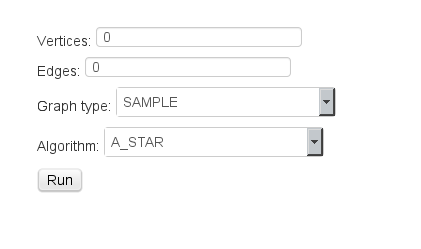
\includegraphics{img/input}
	\caption{Konfiguracja testowa do weryfikacji poprawnej instalacji aplikacji.}
	\label{fig:konfiguracja}
\end{figure}

Rysunek \ref{fig:wyniki} prezentuje wygląd strony z wynikami dla {\it Sample graph} oraz {\it A*}.

\begin{figure}[!h]
	\centering
	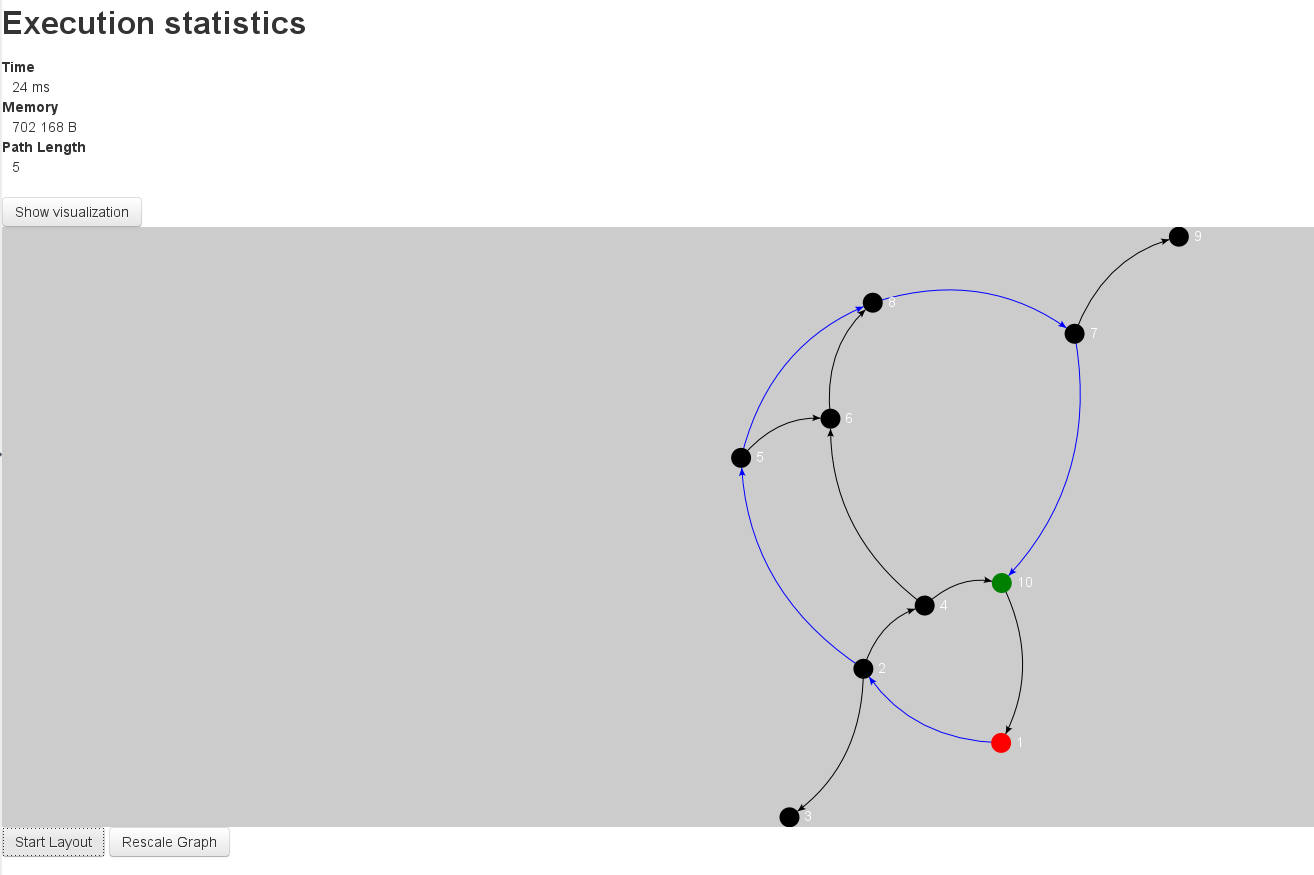
\includegraphics[width=\linewidth]{img/results}
	\caption{Przykładowy wynik planowania.}
	\label{fig:wyniki}
\end{figure}

\nocite{*}

\bibliographystyle{plain}
\bibliography{bibliografia}

\end{document}
